We changed Spark settings only after measuring. Each test ran one day of data on prod, and we
read the time of each stage from the Spark event logs~\cite{spark} (Figure~\ref{fig:perf}).
The panels use two versions of Silver: the \emph{old} one, which read three full Bronze days,
and the \emph{new} one with the read window described below. Panel (a) is the old version on
4~November data. Panel (c) compares the old and the new version on the same day, 6~November.

\begin{figure*}[t]
\centering
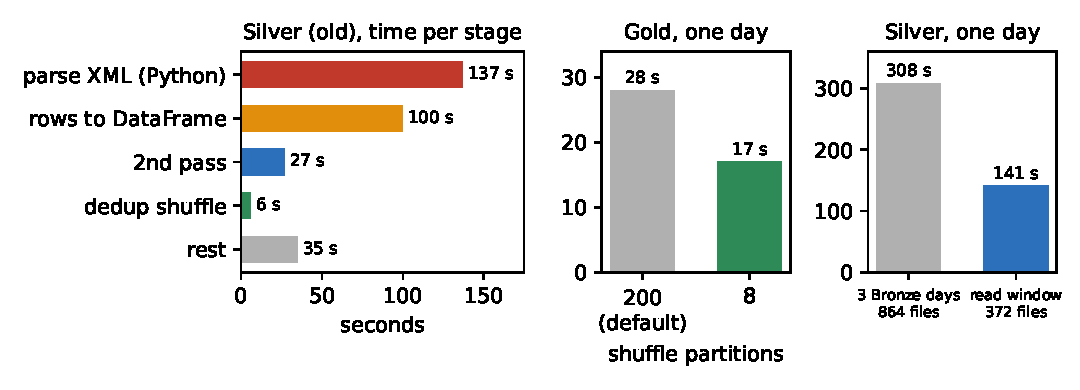
\includegraphics[width=0.7\textwidth]{5_performance.pdf}
\caption{(a) Old Silver (three Bronze days) on 4 November data: time per stage.
(b) Gold for one day with 200 and 8 shuffle partitions.
(c) Old and new Silver on the same day, 6 November: total time.}
\label{fig:perf}
\end{figure*}

\begin{itemize}
  \item \textbf{Gold: 8 shuffle partitions instead of 200.} Gold groups only about 150k rows a
        day, so 200 tasks were mostly overhead. With 8, Gold went from 28\,s to 17\,s.
  \item \textbf{Silver: Spark settings did not help.} The shuffle for removing duplicates takes
        only a few seconds. Most of the time is Python reading the XML files, and each Bronze
        day read costs about 100\,s. So the fix was to read fewer files.
  \item \textbf{Silver: read only the hours it needs.} A night bus that belongs to day $D$ can
        appear in the files of the next UTC day, so the first version read three full Bronze
        days (864 files) to build one day. We checked all 27 days: the stops of day $D$ appear
        from about 23:20 UTC the evening before until at most 01:15 the morning after. With
        2 hours of margin, Silver now reads from 20:00 the evening before to 02:59 the morning
        after (372 files). This cut the run from 308\,s to 141\,s, with exactly the same rows.
        It also makes reruns give the same result, because the old version read up to the
        moment the run started.
  \item \textbf{One Parquet file per day.} Silver and Gold are written with
        \code{repartition("service\_date")}, so each day is one file instead of one per task,
        and later reads open fewer small files. The Silver quality metrics are now computed in
        one aggregation instead of several separate counts.
\end{itemize}

The files between 20:00 and 03:00 UTC are still read by two nightly runs. Saving each parsed
Bronze file once, split by service day, would remove that too; we leave it as future work.
